\chapter{三角函数}
\section{三角函数图象与性质}
\begin{example}
	(1) 将函数 $f(x)=2 \sin 2 x$ 的图象向左平移 $\frac{\pi}{12}$ 个单位长度得到 $g(x)$ 的图象. 若函数 $g(x)$ 在区间 $\left[0, \frac{a}{3}\right],\left[2 a, \frac{7 \pi}{6}\right]$ 上单调增, 求实数 $a$ 的取值范围. (2017 年清华大学 THUSSAT 测试题)

	(2) 已知函数 $f(x)=\sin (\pi x), g(x)=\left\{\begin{array}{ll}\frac{1}{2-2 x}, & x \neq 1, \\ 0, & x=1,\end{array}\right.$ 求函数 $h(x)=f(x)-g(x), x \in(-2,4]$ 的所有零点的和.
\end{example}

\begin{solution}
	(1) 根据题意,
	$$
		g(x)=2 \sin \left(2 x+\frac{\pi}{6}\right)
	$$
	它的单调递增区间为
	$$
		\cdots,\left[-\frac{\pi}{3}, \frac{\pi}{6}\right],\left[\frac{2 \pi}{3}, \frac{7 \pi}{6}\right], \cdots,\left[-\frac{\pi}{3}+k \pi, \frac{\pi}{6}+k \pi\right], k \in \mathbb{N}_{+}
	$$

	于是 $\left\{\begin{array}{l}0<\frac{a}{3} \leqslant \frac{\pi}{6}, \\ -\frac{\pi}{3}+k \pi \leqslant 2 a \leqslant \frac{\pi}{6}+k \pi, \quad k \in \mathbb{N}_{+}\end{array}\right. $

	$\Rightarrow\left\{\begin{array}{l}0<a \leqslant \frac{\pi}{2}, \\ -\frac{\pi}{6}+\frac{k \pi}{2} \leqslant a \leqslant \frac{\pi}{12}+\frac{k \pi}{2}, \quad k \in \mathbb{N}_{+},\end{array}\right.$
	所以
	$$
		\frac{\pi}{3} \leqslant a \leqslant \frac{\pi}{2}
	$$

	所以实数 $a$ 的取值范围是 $\left[\frac{\pi}{3}, \frac{\pi}{2}\right]$.

	(2) 如\autoref{fig:2.1.2},
	\begin{figure}[ht]
		\centering
		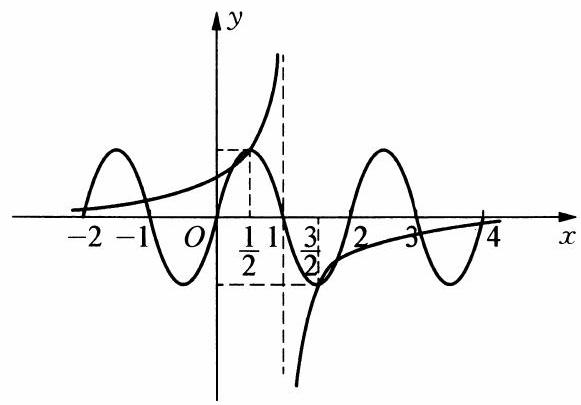
\includegraphics[width=0.5\textwidth]{./images/2.1.1.jpg}
		\caption{}
		\label{fig:2.1.2}
	\end{figure}

	函数 $f(x)$ 和 $g(x)$ 的图象均关于点 $(1,0)$ 对称, 且
	$$
		f\left(\frac{1}{2}\right)=g\left(\frac{1}{2}\right)=1
	$$

	于是函数 $h(x)$ 的零点共有 9 个, 因此所有零点的和为 9 .
\end{solution}

\begin{note}
	第(1)小题也可以直接由 $0<\frac{a}{3} \leqslant \frac{\pi}{6}$, 及 $\frac{2 \pi}{3} \leqslant 2 a \leqslant \frac{7 \pi}{6}$ 得出结论.第 (2) 小题对于零点的个数常结合图象求之. 本题关键是注意到 $f(x)$ 与 $g(x)$均关于点 $(1,0)$ 对称.
\end{note}

\begin{example}
	设函数 $f(x)=|\sin x|+|\cos x|$.

	(1) 试讨论函数的性质(有界性, 奇偶性, 单调性, 周期性), 求出其最值, 并作出其在 $[0,2 \pi]$ 上的图象;

	(2) 求函数 $y=\sqrt{\sin x}+\sqrt{\cos x}\left(x \in\left[0, \frac{\pi}{2}\right]\right)$ 的值域. (2007 年上海交大自主招生)

\end{example}
\begin{solution}
	(1) 因为
	$$
		f(-x)=|\sin (-x)|+|\cos (-x)|=|\sin x|+|\cos x|=f(x)
	$$
	所以这是一个偶函数.
	$$
		\begin{aligned}
			f\left(x+\frac{\pi}{2}\right) & =\left|\sin \left(x+\frac{\pi}{2}\right)\right|+\left|\cos \left(x+\frac{\pi}{2}\right)\right| \\
			                              & =|\cos x|+|\sin x|=f(x)
		\end{aligned}
	$$
	所以这是一个周期为 $\frac{\pi}{2}$ 的周期函数.
	$$
		2=2\left(\sin ^{2} x+\cos ^{2} x\right) \geqslant f^{2}(x) \geqslant \sin ^{2} x+\cos ^{2} x=1
	$$
	所以 $1 \leqslant f(x) \leqslant \sqrt{2}$, 所以 $f(x)$ 有上下界. 而当 $x=0$, 或 $\frac{\pi}{2}$ 时, $f(x)=1$;\\
	$x=\frac{\pi}{4}$ 时, $f(x)=\sqrt{2}$. 所以 $f(x)$ 的最小值为 1 , 最大值为 $\sqrt{2}$.

	由于 $f(x)$ 是一个周期为 $\frac{\pi}{2}$ 的周期函数, 所以我们只需要考查它在 $\left(0, \frac{\pi}{2}\right)$ 上的单调性即可.

	此时
	$f(x)=\sin x+\cos x=\sqrt{2} \sin \left(x+\frac{\pi}{4}\right)$,
	那么 $f(x)$ 在 $\left(\frac{k \pi}{2}, \frac{k \pi}{2}+\frac{\pi}{4}\right)(k \in \mathbb{Z})$ 上递增,在 $\left(\frac{k \pi}{2}+\frac{\pi}{4}, \frac{k \pi}{2}+\frac{\pi}{2}\right)(k \in \mathbb{Z})$ 上递减.

	图像如\autoref{fig:2.1.2}所示.
	\begin{figure}[ht]
		\centering
		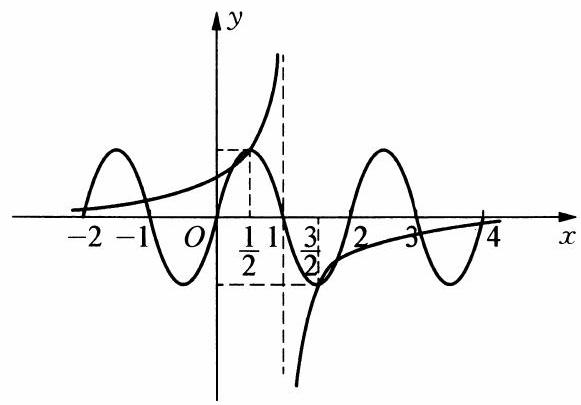
\includegraphics[width=0.35\textwidth]{./images/2.1.2.jpg}
		\caption{}
		\label{fig:2.1.2}
	\end{figure}

	(2) 因为 $x \in\left[0, \frac{\pi}{2}\right]$, 所以 $0 \leqslant \sin x \leqslant 1,0 \leqslant \cos x \leqslant 1$.

	所以 $\sqrt{\sin x} \geqslant \sin x \geqslant \sin ^{2} x, \sqrt{\cos x} \geqslant \cos x \geqslant \cos ^{2} x$.

	所以 $\sqrt{\sin x}+\sqrt{\cos x} \geqslant \sin x+\cos x \geqslant \sin ^{2} x+\cos ^{2} x \geqslant 1$.

	且当 $x=0$,或 $\frac{\pi}{2}$ 时, $\sqrt{\sin x}+\sqrt{\cos x}=1$.

	另一方面, 由

	$$
		\begin{aligned}
			(\sqrt{\sin x}+\sqrt{\cos x})^{2} & =\sin x+\cos x+2 \sqrt{\sin x \cos x}                         \\
			                                  & =\sqrt{2} \sin \left(x+\frac{\pi}{4}\right)+\sqrt{2 \sin 2 x} \\
			                                  & \leqslant 2 \sqrt{2}
		\end{aligned}
	$$

	所以

	$\sqrt{\sin x}+\sqrt{\cos x} \leqslant 2^{\frac{3}{4}}$.

	且当 $x=\frac{\pi}{4}$ 时, $\sqrt{\sin x}+\sqrt{\cos x}=2^{\frac{3}{4}}$.

	所以函数 $y=\sqrt{\sin x}+\sqrt{\cos x}\left(x \in\left[0, \frac{\pi}{2}\right]\right)$ 的值域为 $\left[1,2^{\frac{3}{4}}\right]$.
\end{solution}
\begin{note}
	这两道题都是考查三角函数的基本性质. 第(1)小题关键是如何看出 $\frac{\pi}{2}$ 是函数的周期, 实际上可用图象分析出来, 或者取特殊点观察可得. 第 (2) 小题求值域方法很多, 关键是细心谨慎, 小心放缩. 本小题还可用均值不等式, 柯西不等式来求解.\\
\end{note}

\begin{example}
	已知函数 $f(x)=\tan \left(\frac{\pi}{\sqrt{3}} \sin x\right)$.

	(1) 求 $f(x)$ 的定义域和值域;

	(2) 在 $(-\pi, \pi)$ 中, 求 $f(x)$ 的单调区间;

	(3) 判定方程 $f(x)=\tan \frac{\sqrt{2}}{3} \pi$ 在区间 $(-\pi, \pi)$ 上解的个数.
\end{example}
\begin{solution}
	(1) 因为 $-1 \leqslant \sin x \leqslant 1$, 所以 $-\frac{\pi}{\sqrt{3}} \leqslant \frac{\pi}{\sqrt{3}} \sin x \leqslant \frac{\pi}{\sqrt{3}}$.

	又因为函数 $y=\tan x$ 在 $x=k \pi+\frac{\pi}{2}(k \in \mathbb{Z})$ 处无定义, 且

	$$
		\left(-\frac{\pi}{2}, \frac{\pi}{2}\right) \varsubsetneqq\left[-\frac{\pi}{\sqrt{3}}, \frac{\pi}{\sqrt{3}}\right] \varsubsetneqq(-\pi, \pi)
	$$

	所以令 $\frac{\pi}{\sqrt{3}} \sin x= \pm \frac{\pi}{2}$, 则 $\sin x= \pm \frac{\sqrt{3}}{2}$, 解之得: $x=k \pi \pm \frac{\pi}{3}(k \in \mathbb{Z})$.

	所以 $f(x)$ 的定义域是 $A=\left\{x \mid x \in \mathbb{R}\right.$, 且 $\left.x \neq k \pi \pm \frac{\pi}{3}, k \in \mathbb{Z}\right\}$.

	因为 $\tan x$ 在 $\left(-\frac{\pi}{2}, \frac{\pi}{2}\right)$ 内的值域为 $(-\infty,+\infty)$, 而当 $x \in A$ 时, 函数 $y=\tan \left(\frac{\pi}{\sqrt{3}} \sin x\right)$ 的值域 $B$ 满足 $\left(-\frac{\pi}{2}, \frac{\pi}{2}\right) \varsubsetneqq B$, 所以 $f(x)$ 的值域是 $(-\infty,+\infty)$.

	(2) 由 $f(x)$ 的定义域知, $f(x)$ 在 $[0, \pi)$ 中的 $x=\frac{\pi}{3}$ 和 $x=\frac{2 \pi}{3}$ 处无定义.设 $t=\frac{\pi}{\sqrt{3}} \sin x$, 则当 $x \in\left[0, \frac{\pi}{3}\right) \cup\left(\frac{\pi}{3}, \frac{2 \pi}{3}\right) \cup\left(\frac{2 \pi}{3}, \pi\right)$ 时, $t \in$ $\left[0, \frac{\pi}{2}\right) \cup\left(\frac{\pi}{2}, \frac{\pi}{\sqrt{3}}\right]$, 且以 $t$ 为自变量的函数 $y=\tan t$ 在区间 $\left(0, \frac{\pi}{2}\right)$, $\left(\frac{\pi}{2}, \frac{\pi}{\sqrt{3}}\right]$ 上分别单调递增.

				又因为当 $x \in\left[0, \frac{\pi}{3}\right)$ 时, 函数 $t=\frac{\pi}{\sqrt{3}} \sin x$ 单调递增, 且 $t \in\left[0, \frac{\pi}{2}\right)$;当 $x \in\left(\frac{\pi}{3}, \frac{\pi}{2}\right]$ 时, 函数 $t=\frac{\pi}{\sqrt{3}} \sin x$ 单调递增, 且 $t \in\left(\frac{\pi}{2}, \frac{\pi}{\sqrt{3}}\right]$;

			当 $x \in\left[\frac{\pi}{2}, \frac{2 \pi}{3}\right)$ 时, 函数 $t=\frac{\pi}{\sqrt{3}} \sin x$ 单调递减, 且 $t \in\left(\frac{\pi}{2}, \frac{\pi}{\sqrt{3}}\right]$;\\
	当 $x \in\left(\frac{2 \pi}{3}, \pi\right)$ 时, 函数 $t=\frac{\pi}{\sqrt{3}} \sin x$ 单调递减, 且 $t \in\left(0, \frac{\pi}{2}\right)$.

	所以 $f(x)=\tan \left(\frac{\pi}{\sqrt{13}} \sin x\right)$ 在区间 $\left[0, \frac{\pi}{3}\right),\left(\frac{\pi}{3}, \frac{\pi}{2}\right]$ 上分别是单调递增函数; 在 $\left[\frac{\pi}{2}, \frac{2 \pi}{3}\right),\left(\frac{2 \pi}{3}, \pi\right)$ 上是单调递减函数.

				又 $f(x)$ 是奇函数, 所以区间 $\left(-\frac{\pi}{3}, 0\right],\left[-\frac{\pi}{2},-\frac{\pi}{3}\right)$ 也是 $f(x)$ 的单调递增区间, $\left(-\pi,-\frac{2 \pi}{3}\right),\left(-\frac{2 \pi}{3},-\frac{\pi}{2}\right]$ 是 $f(x)$ 的单调递减区间.

	故在 $(-\pi, \pi)$ 中, $f(x)$ 的单调递增区间为:

	$$
		\left[-\frac{\pi}{2},-\frac{\pi}{3}\right),\left(-\frac{\pi}{3}, \frac{\pi}{3}\right),\left(\frac{\pi}{3}, \frac{\pi}{2}\right]
	$$

	单调递减区间为:

	$$
		\left(-\pi,-\frac{2 \pi}{3}\right),\left(-\frac{2 \pi}{3},-\frac{\pi}{2}\right],\left[\frac{\pi}{2}, \frac{2 \pi}{3}\right),\left(\frac{2 \pi}{3}, \pi\right)
	$$

	(3) 由 $f(x)=\tan \frac{\sqrt{2}}{3} \pi$, 得 $\tan \left(\frac{\pi}{\sqrt{3}} \sin x\right)=\tan \left(\frac{\sqrt{2}}{3} \pi\right)$


	\begin{align*}
		 & \Leftrightarrow \frac{\pi}{\sqrt{3}} \sin x=k \pi+\frac{\sqrt{2}}{3} \pi(k \in \mathbb{Z}) \\
		 & \Leftrightarrow \sin x=k \sqrt{3}+\frac{\sqrt{6}}{3}(k \in \mathbb{Z}) \tag{1}
	\end{align*}


	又因为 $-1 \leqslant \sin x \leqslant 1, \frac{-\sqrt{3}-\sqrt{2}}{3} \leqslant k \leqslant \frac{\sqrt{3}-\sqrt{2}}{3}$, 所以 $k=0$ 或 $k=-1$.当 $k=0$ 时, 从 (1)得方程 $\sin x=\frac{\sqrt{6}}{3}$;

	当 $k=1$ 时, 从(1)得方程 $\sin x=-\sqrt{3}+\frac{\sqrt{6}}{3}$.

	显然方程 $\sin x=\frac{\sqrt{6}}{3}, \sin x=-\sqrt{3}+\frac{\sqrt{6}}{3}$, 在 $(-\pi, \pi)$ 上各有两个解, 故 $f(x)=\tan \frac{\sqrt{2}}{3} \pi$ 在区间 $(-\pi, \pi)$ 上共有 4 个解.
\end{solution}
\begin{note}
	本题是正弦函数与正切函数的复合. (1) 求 $f(x)$ 的定义域和值域,应当先搞清楚 $y=\frac{\pi}{\sqrt{3}} \sin x$ 的值域与 $y=\tan x$ 的定义域的交集; (2)求 $f(x)$\\
	的单调区间, 必须先搞清 $f(x)$ 的基本性质, 如奇偶性, 周期性, 复合函数单调性等.
\end{note}

\begin{example}
	设 $\omega$ 为正实数, 若存在 $a ,  b(\pi \leqslant a<b \leqslant 2 \pi)$, 使得 $\sin \omega a+\sin \omega b$ $=2$. 求 $\omega$ 的取值范围. (2015 年全国高中数学联赛)
\end{example}
\begin{solution}
	由 $\sin \omega a+\sin \omega b=2$ 知, $\sin \omega a=\sin \omega b=1$, 而 $[\omega a, \omega b] \subseteq[\omega \pi$, $2 \omega \pi]$, 故题目条件等价于: 存在整数 $k ,  l(k<l)$, 使得

	\begin{equation*}
		\omega \pi \leqslant 2 k \pi+\frac{\pi}{2}<2 l \pi+\frac{\pi}{2} \leqslant 2 \omega \pi \tag{1}
	\end{equation*}

	当 $\omega \geqslant 4$ 时, 区间 $[\omega \pi, 2 \omega \pi]$ 的长度不小于 $4 \pi$, 故必存在 $k ,  l$ 满足 (1) 式.

	当 $0<\omega<4$ 时, 注意到 $[\omega \pi, 2 \omega \pi] \subseteq(0,8 \pi)$, 故仅需考虑如下几种情况:

	(1) $\omega \pi \leqslant \frac{\pi}{2}<\frac{5 \pi}{2} \leqslant 2 \omega \pi$, 此时有 $\omega \leqslant \frac{1}{2}$, 且 $\omega \geqslant \frac{5}{4}$, 无解;

	(2) $\omega \pi \leqslant \frac{5 \pi}{2}<\frac{9 \pi}{2} \leqslant 2 \omega \pi$, 此时有 $\frac{9}{4} \leqslant \omega \leqslant \frac{5}{2}$;

	(3) $\omega \pi \leqslant \frac{9 \pi}{2}<\frac{13 \pi}{2} \leqslant 2 \omega \pi$, 此时有 $\frac{13}{4} \leqslant \omega \leqslant \frac{9}{2}$, 得 $\frac{13}{4} \leqslant \omega<4$.

	综合 (1), (2), (3) 及 $\omega \geqslant 4$ 得, $\omega$ 的取值范围是
	$$
		\left\{\omega \left\lvert\, \frac{9}{4} \leqslant \omega \leqslant \frac{5}{2}\right. \text {, 或 } \omega \geqslant \frac{13}{4}\right\} .
	$$
\end{solution}
\begin{note}
	本题难点在于分类讨论. 首先注意到 $\omega \geqslant 4$ 时, 区间 $[\omega \pi, 2 \omega \pi]$ 的长度大于或等于 $4 \pi$, 在两个周期之内. 一定存在两个最大值, 其次逐步对取得 1 时, $\omega a ,  \omega b$ 的相应值加以讨论.
\end{note}

\begin{example}
	设函数 $f(x)=\sin ^{2} x+(2 a-1) \sin x+a^{2}+\frac{1}{4}$, 已知 $x \in$ $\left[\frac{5}{6} \pi, \frac{3}{2} \pi\right]$, 求 $f(x)$ 的最值.
\end{example}
\begin{solution}
	设 $\sin x=t$, 则 $t \in\left[-1, \frac{1}{2}\right]$.

	$f(x)=g(t)=t^{2}+(2 a-1) t+a^{2}+\frac{1}{4}$, 对称轴为 $t=\frac{1-2 a}{2}$.

	当 $\frac{1-2 a}{2} \leqslant-1$ 即 $a \geqslant \frac{3}{2}$ 时, $\left[-1, \frac{1}{2}\right]$ 为 $g(t)$ 的单调增区间,所以

	$$
		f_{\min }=g(-1)=a^{2}-2 a+\frac{9}{4}, f_{\max }=g\left(\frac{1}{2}\right)=a^{2}+a
	$$

	当 $-1<\frac{1-2 a}{2} \leqslant-\frac{1}{4}$ 即 $\frac{3}{4} \leqslant a<\frac{3}{2}$ 时, $g(-1) \leqslant g\left(\frac{1}{2}\right)$, 所以

	$$
		f_{\min }=g\left(\frac{1-2 a}{2}\right)=a, f_{\max }=g\left(\frac{1}{2}\right)=a^{2}+a
	$$

	当 $-\frac{1}{4}<\frac{1-2 a}{2} \leqslant \frac{1}{2}$ 即 $0 \leqslant a<\frac{3}{4}$ 时, $g(-1)>g\left(\frac{1}{2}\right)$, 所以

	$$
		f_{\min }=g\left(\frac{1-2 a}{2}\right)=a, f_{\max }=g(-1)=a^{2}-2 a+\frac{9}{4}
	$$

	当 $\frac{1-2 a}{2}>\frac{1}{2}$ 即 $a<0$ 时, $\left[-1, \frac{1}{2}\right]$ 为 $g(t)$ 的单调减区间, 所以

	$$
		f_{\min }=g\left(\frac{1}{2}\right)=a^{2}+a, f_{\max }=g(-1)=a^{2}-2 a+\frac{9}{4}
	$$
\end{solution}
\begin{note}
	求形如 $f(x)=A \sin ^{2} x+B \sin x+C$ 形式的最值, 通常用换元法,化成二次函数在区间的最值问题.
\end{note}

\begin{example}
	已知函数 $f(x)=\frac{a-2 \cos x}{3 \sin x}$ 在区间 $\left(0, \frac{\pi}{2}\right)$ 内是增函数, 求 $a$ 的取值范围.
\end{example}
\begin{analysis}
	根据增函数的定义,列出不等式,求 $a$ 的取值范围.
\end{analysis}
\begin{solution}
	解法一: 由条件得: 当 $0<x_{1}<x_{2}<\frac{\pi}{2}$ 时,
	$$
		f\left(x_{1}\right)-f\left(x_{2}\right)=\frac{a-2 \cos x_{1}}{3 \sin x_{1}}-\frac{a-2 \cos x_{2}}{3 \sin x_{2}}<0
	$$

	因为 $\sin x_{2}>\sin x_{1}>0$, 所以去分母得
	$$
		a \sin x_{2}-2 \cos x_{1} \sin x_{2}-a \sin x_{1}+2 \cos x_{2} \sin x_{1}<0,
	$$

	整理得
	$$
		a\left(\sin x_{2}-\sin x_{1}\right)-2 \sin \left(x_{2}-x_{1}\right)<0,
	$$

	故
	$a<\frac{2 \sin \left(x_{2}-x_{1}\right)}{\sin x_{2}-\sin x_{1}}=\frac{4 \sin \frac{x_{2}-x_{1}}{2} \cos \frac{x_{2}-x_{1}}{2}}{2 \cos \frac{x_{2}+x_{1}}{2} \sin \frac{x_{2}-x_{1}}{2}}=\frac{2 \cos \frac{x_{2}-x_{1}}{2}}{\cos \frac{x_{2}+x_{1}}{2}}$

	由于
	\begin{align}
		\cos \frac{x_{2}-x_{1}}{2} & =\cos \frac{x_{2}}{2} \cos \frac{x_{1}}{2}+\sin \frac{x_{2}}{2} \sin \frac{x_{1}}{2} \\
		                           & >\cos \frac{x_{2}}{2} \cos \frac{x_{1}}{2}-\sin \frac{x_{2}}{2} \sin \frac{x_{1}}{2} \\
		                           & =\cos \frac{x_{1}+x_{2}}{2}>0
	\end{align}

	所以 $\frac{\cos \frac{x_{2}-x_{1}}{2}}{\cos \frac{x_{1}+x_{2}}{2}}>1$, 从而 $a \leqslant 2$, 即 $a$ 的取值范围为 $(-\infty, 2]$.

	解法二:记 $\tan \frac{x}{2}=t$, 则 $\sin x=\frac{2 t}{1+t^{2}}, \cos x=\frac{1-t^{2}}{1+t^{2}}$, 且 $t \in(0,1)$,

	所以
	$$
		\begin{aligned}
			g(t) & =f(x)=\frac{a-2 \times \frac{1-t^{2}}{1+t^{2}}}{3 \times \frac{2 t}{1+t^{2}}}=\frac{(a-2)+(a+2) t^{2}}{6 t} \\
			     & =\frac{a-2}{6 t}+\frac{a+2}{6} \cdot t
		\end{aligned}
	$$

	设 $0<t_{1}<t_{2}<1$ , 则
	$$
		g\left(t_{1}\right)-g\left(t_{2}\right)=\left(\frac{a-2}{6 t_{1}}+\frac{a+2}{6} t_{1}\right)-\left(\frac{a-2}{6 t_{2}}+\frac{a+2}{6} t_{2}\right)<0
	$$

	去分母得
	$$
		(a-2) t_{2}+(a+2) t_{1}^{2} t_{2}-(a-2) t_{1}-(a+2) t_{1} t_{2}^{2}<0
	$$

	整理得
	$$
		\left(t_{2}-t_{1}\right)\left(a-a t_{1} t_{2}-2-2 t_{1} t_{2}\right)<0
	$$

	而 $0<t_{1}<t_{2}<1$, 所以 $a<\frac{2\left(1+t_{1} t_{2}\right)}{1-t_{1} t_{2}}$.

	显然 $\frac{1+t_{1} t_{2}}{1-t_{1} t_{2}}>1$, 故 $a \leqslant 2$, 即 $a$ 的取值范围为 $(-\infty, 2]$.
\end{solution}
\begin{note}
	对于含参数不等式的问题, 如 $a<f(t)$ 恒成立, 则应取 $f(t)$ 的最小值后得 $a$ 的取值范围; 如 $a>f(t)$, 则取 $f(t)$ 的最大值后得 $a$ 的取值范围,如 $f(t)$ 无最值, 则取它的变化趋势的最值.
\end{note}

\begin{example}
	设函数 $f(x), g(x)$ 对任意实数 $x$ 均有 $-\frac{\pi}{2}<f(x)+g(x)<\frac{\pi}{2}$,并且 $-\frac{\pi}{2}<f(x)-g(x)<\frac{\pi}{2}$. 求证: 对任意实数 $x$ 均有 $\cos f(x)>$ $\sin g(x)$, 并由此证明: 对任意实数 $x$ 均有 $\cos (\cos x)>\sin (\sin x)$.
\end{example}
\begin{proof}
	由条件可得 $-\frac{\pi}{2}<f(x)<\frac{\pi}{2},-\frac{\pi}{2}<g(x)<\frac{\pi}{2}$.

	若 $0 \leqslant f(x)<\frac{\pi}{2}$, 得到 $-\frac{\pi}{2}<g(x)<\frac{\pi}{2}-f(x) \leqslant \frac{\pi}{2}$, 由于 $y=\sin x$\\
	在 $\left[-\frac{\pi}{2}, \frac{\pi}{2}\right]$ 上为单调增函数, 故 $\sin g(x)<\sin \left[\frac{\pi}{2}-f(x)\right]=\cos f(x)$.

	若 $-\frac{\pi}{2}<f(x)<0$, 则由条件 $-\frac{\pi}{2}<g(x)<\frac{\pi}{2}+f(x)<\frac{\pi}{2}$, 同样由 $y=\sin x$ 在 $\left[-\frac{\pi}{2}, \frac{\pi}{2}\right]$ 上为单调增函数, 故
	$$
		\sin g(x)<\sin \left[\frac{\pi}{2}+f(x)\right]=\cos f(x)
	$$

	对任意实数 $x$, 均有
	$$
		|\cos x \pm \sin x|=\sqrt{2}\left|\sin \left(\frac{\pi}{4} \pm x\right)\right| \leqslant \sqrt{2}<\frac{\pi}{2}
	$$

	根据已证的不等式, 就有 $\cos (\cos x)>\sin (\sin x)$.
\end{proof}
\begin{note}
	利用正, 余弦函数的单调性, 结合正, 余弦函数的有界性以及上述结论, 我们还有如下的一些结论: $\sin (\cos x)<\cos (\sin x), \sin (\sin (\sin x))<$ $\sin (\cos (\cos x))<\cos (\cos (\cos x))$ 等.
\end{note}

\begin{example}
	已知 $f(x)=a x+\sin x$ 表示的图象上有两条切线相互垂直, 求 $a$的值. (2010 北大保送生考试)
\end{example}
\begin{solution}
	$f(x)=a x+\sin x \Rightarrow f^{\prime}(x)=a+\cos x$, 从而如果有两条切线垂直,那么存在这样的 $x_{1}, x_{2}$ 使得 $\left(a+\cos x_{1}\right)\left(a+\cos x_{2}\right)=-1$, 从函数图象来看,一个二次函数的两个根都在 $(-1,1)$ 上, 首项系数为 1 , 并且开口朝上, 可以感觉到能取到的最小值只有在尽量的往下移动, 也就是在两个根分别是 $-1,1$ 的时候最小值可以尽可能的小, 此时刚好等于 -1 , 因此可以感觉到这道题实际上卡得很死 (指的中间的放缩), 我们具体的操作如下:

	不妨设 $\cos x_{1} \leqslant \cos x_{2},\left(a+\cos x_{1}\right)\left(a+\cos x_{2}\right)<0$, 从而 $a \in\left(-\cos x_{2}\right.$, $-\cos x_{1}$ ), 此时可以得到 $0<a+\cos x_{2} \leqslant a+1, a-1 \leqslant a+\cos x_{1}<0$, 那么
	$$
		-1=\left(a+\cos x_{1}\right)\left(a+\cos x_{2}\right) \geqslant(a+1)(a-1)=a^{2}-1 \geqslant-1
	$$
	所以中间不等号必须全部取等号, 此时只能 $a=0$, 并且在 $x_{1}=\pi, x_{2}=$ 0 的时候两个点的切线互相垂直.
\end{solution}
\begin{note}
	本题是挺不错的一道题, 考查学生对函数基本性质的理解. 实际上在得出结论之前, 如果能够想象出图象是最好了, 这样会对最后结果的把握很有帮助, 具体的分析都比较常规, 没必要细讲. 但是要注意一个陷阱, 有些学生的做法会存在逻辑问题,并没有真的得出 $a=0$, 可以给学生强调这一点, 这种题每一步的逻辑要对.
\end{note}

\begin{example}
	证明函数 $g(x)=\cos \sqrt[3]{x}$ 不是周期函数.
\end{example}
\begin{analysis}
	当结论出现否定的形式时,宜采用反证法.
\end{analysis}
\begin{proof}
	假设 $g(x)$ 是周期函数, 非零常数 $T$ 是它的一个周期, 则 $\cos \sqrt[3]{x+T}=\cos \sqrt[3]{x}$ 对一切实数 $x$ 都成立. 取 $x=0$, 得 $\cos \sqrt[3]{T}=1$, 从而 $\sqrt[3]{T}=2 k \pi(k \neq 0, k \in \mathbb{Z})$.

	取 $x=T$, 得 $\cos \sqrt[3]{2 T}=\cos \sqrt[3]{T}=1$, 有 $\sqrt[3]{2 T}=2 e \pi(e \neq 0, e \in \mathbb{Z})$. 于是 $\frac{\sqrt[3]{2 T}}{\sqrt[3]{T}}=\frac{2 e \pi}{2 k \pi}=\frac{e}{k}$, 即 $\sqrt[3]{2}=\frac{e}{k}$, 从而 $\sqrt[3]{2}$ 是有理数, 这与 $\sqrt[3]{2}$ 是无理数相矛盾,故函数 $g(x)=\cos \sqrt[3]{x}$ 不是周期函数.
\end{proof}
\begin{note}
	当结论是肯定或否定形式, 含有“至多”, “至少”等字样时, 可利用反证法证明问题. 又如: 求证函数 $y=|\sin x|+|\cos x|$ 的最小正周期是 $\frac{\pi}{2}$.

	易知 $\frac{\pi}{2}$ 是它的周期, 再证 $\frac{\pi}{2}$ 是它的最小正周期. 假设 $0<T<\frac{\pi}{2}$ 是 $y=$ $|\sin x|+|\cos x|$ 的周期, 则 $|\sin (x+T)|+|\cos (x+T)|=|\sin x|+$ $|\cos x|$ 对任意 $x$ 都成立, 于是取 $x=0$, 得 $|\sin T|+|\cos T|=|\sin 0|+$ $|\cos 0|=1$, 但 $|\sin T|+|\cos T|=\sin T+\cos T=\sqrt{2} \sin \left(T+\frac{\pi}{4}\right)>1$, 故矛盾,所以 $T$ 不存在,原命题正确.
\end{note}

\begin{example}
	如果圆 $x^{2}+y^{2}=k^{2}$ 至少覆盖函数 $f(x)=\sqrt{3} \sin \frac{\pi x}{k}$ 的一个最大值点和一个最小值点. 试求 $k$ 的取值范围.
\end{example}
\begin{solution}
	因为 $f(x)=\sqrt{3} \sin \frac{\pi x}{k}$ 为奇函数, 图象关于原点对称, 故只需要已知圆 $x^{2}+y^{2}=k^{2}$ 覆盖 $f(x)$ 的一个最值点即可. 令 $\frac{\pi x}{k}=\frac{\pi}{2}$, 解得 $f(x)$ 的距原点最近的一个最大值点为 $P\left(\frac{k}{2}, \sqrt{3}\right)$, 依题意
	$$
		k^{2} \geqslant\left(\frac{k}{2}\right)^{2}+(\sqrt{3})^{2}
	$$
	解得 $|k| \geqslant 2$.

	所以 $k$ 的取值范围是 $(-\infty,-2] \cup[2,+\infty)$.
\end{solution}
\begin{note}
	本题巧妙运用函数的奇偶性, 将问题简化为覆盖一个最大点, 这种利用三角函数的奇偶性简化解题的方法是解三角函数性质题的常用\\
	方法.
\end{note}

\begin{example}
	求函数 $y=(a+\cos x)(a+\sin x)$ 的值域.
\end{example}
\begin{analysis}
	对于含参数的函数, 应对 $a$ 进行分类讨论.
\end{analysis}
\begin{solution}
	$$
		y=a^{2}+a(\sin x+\cos x)+\sin x \cos x
	$$
	设 $\sin x+\cos x=t$, 则 $\sin x \cos x=\frac{t^{2}-1}{2},-\sqrt{2} \leqslant t \leqslant \sqrt{2}$, 所以
	$$
		y=a^{2}+a t+\frac{1}{2}\left(t^{2}-1\right)=\frac{1}{2}(t+a)^{2}+\frac{a^{2}-1}{2}
	$$

	(1) 当 $a \geqslant \sqrt{2}$ 时, 当 $t=\sqrt{2}$ 时, $y_{\text {max }}=a^{2}+\sqrt{2} a+\frac{1}{2}=\left(a+\frac{\sqrt{2}}{2}\right)^{2}$;当 $t=-\sqrt{2}$ 时, $y_{\text {min }}=a^{2}-\sqrt{2} a+\frac{1}{2}=\left(a-\frac{\sqrt{2}}{2}\right)^{2}$.

	所以函数的值域为 $\left[\left(a-\frac{\sqrt{2}}{2}\right)^{2},\left(a+\frac{\sqrt{2}}{2}\right)^{2}\right]$.

	(2) 当 $0 \leqslant a \leqslant \sqrt{2}$ 时, 当 $t=\sqrt{2}$ 时, $y_{\text {max }}=\left(a+\frac{\sqrt{2}}{2}\right)^{2}$;

	当 $t=-a$ 时, $y_{\text {min }}=\frac{a^{2}-1}{2}$.

	所以函数的值域为 $\left[\frac{a^{2}-1}{2},\left(a+\frac{\sqrt{2}}{2}\right)^{2}\right]$.

	(3) 当 $-\sqrt{2} \leqslant a \leqslant 0$ 时, 当 $t=-\sqrt{2}$ 时, $y_{\text {max }}=\left(a-\frac{\sqrt{2}}{2}\right)^{2}$;

	当 $t=-a$ 时, $y_{\text {min }}=\frac{a^{2}-1}{2}$.

	所以函数的值域为 $\left[\frac{a^{2}-1}{2},\left(a-\frac{\sqrt{2}}{2}\right)^{2}\right]$.

	(4) 当 $a<-\sqrt{2}$ 时, 当 $t=-\sqrt{2}$ 时, $y_{\text {max }}=\left(a-\frac{\sqrt{2}}{2}\right)^{2}$;

	当 $t=\sqrt{2}$ 时, $y_{\text {min }}=\left(a+\frac{\sqrt{2}}{2}\right)^{2}$.

	所以函数的值域为 $\left[\left(a+\frac{\sqrt{2}}{2}\right)^{2},\left(a-\frac{\sqrt{2}}{2}\right)^{2}\right]$.
\end{solution}
\begin{note}
	有关含 $\sin x$ 和 $\cos x$ 的二次函数值域问题, 必须注意隐含条件 $|\sin x| \leqslant 1$ 和 $|\cos x| \leqslant 1$.
\end{note}

\begin{example}
	设函数 $f(x)$ 的定义域为 $\mathbb{R}$, 对任意实数 $\alpha ,  \beta$ 有
	$$
		f(\alpha)+f(\beta)=2 f\left(\frac{\alpha+\beta}{2}\right) f\left(\frac{\alpha-\beta}{2}\right) \text {, 且 } f\left(\frac{\pi}{3}\right)=\frac{1}{2}, f\left(\frac{\pi}{2}\right)=0 \text {. }
	$$
	(1) 求证: $f(-x)=f(x)=-f(\pi-x)$;

	(2) 若 $0 \leqslant x<\frac{\pi}{2}$ 时, $f(x)>0$, 求证: $f(x)$ 在 $[0, \pi]$ 上单调递减;

	(3) 求 $f(x)$ 的最小周期并加以证明.
\end{example}
\begin{analysis}
	正确理解所给等式, 通过赋值法, 定义法解答本题.
\end{analysis}
\begin{solution}
	(1) 因为 $f\left(\frac{\pi}{3}\right)+f\left(\frac{\pi}{3}\right)=2 f\left(\frac{\pi}{3}\right) f(0)$, 且 $f\left(\frac{\pi}{3}\right)=\frac{1}{2}$, 所以 $f(0)=1$.

	又 $f(x)+f(-x)=2 f(0) f(x)$, 故 $f(x)=f(-x)$.

	又由于 $f(x)+f(\pi-x)=2 f\left(\frac{\pi}{2}\right) f\left(x-\frac{\pi}{2}\right)$, 且 $f\left(\frac{\pi}{2}\right)=0$, 故有
	$$
		f(x)=f(-x)=-f(\pi-x)
	$$

	(2) 由 $f(-x)=f(x)$ 且 $0 \leqslant x<\frac{\pi}{2}$ 时, $f(x)>0$, 得当 $-\frac{\pi}{2}<x<\frac{\pi}{2}$时, $f(x)>0$.

	设 $0 \leqslant x_{1}<x_{2} \leqslant \pi$, 则
	$$
		\begin{aligned}
			f\left(x_{1}\right)-f\left(x_{2}\right) & =f\left(x_{1}\right)+f\left(\pi-x_{2}\right)                                       \\
			                                        & =2 f\left(\frac{x_{1}+\pi-x_{2}}{2}\right) f\left(\frac{x_{1}+x_{2}-\pi}{2}\right)
		\end{aligned}
	$$

	因为 $0 \leqslant \frac{x_{1}-x_{2}+\pi}{2}<\frac{\pi}{2},-\frac{\pi}{2}<\frac{x_{1}+x_{2}-\pi}{2}<\frac{\pi}{2}$, 所以
	$$
		f\left(\frac{x_{1}+\pi-x_{2}}{2}\right)>0, f\left(\frac{x_{1}+x_{2}-\pi}{2}\right)>0
	$$

	从而 $f\left(x_{1}\right)>f\left(x_{2}\right)$, 即 $f(x)$ 在 $[0, \pi]$ 上单调递减.

	(3) 由 (1) $f(-x)=-f(\pi-x)$, 得

	$$
		f(x)=-f(\pi+x), f(\pi+x)=-f(2 \pi+x)
	$$

	所以 $f(2 \pi+x)=f(x)$, 说明 $2 \pi$ 是原函数的一个周期.

	假设 $T_{0}$ 也是原函数的一个周期, 且 $T_{0} \in(0,2 \pi)$, 则由 $f\left(T_{0}+x\right)=$ $f(x)$, 得 $f(0)=f\left(T_{0}\right)$.

	但若 $T_{0} \in(0, \pi]$ 时, 因原函数是单调递减函数, 所以 $f(0)>f\left(T_{0}\right)$, 两\\
	者矛盾;

	若 $T_{0} \in(\pi, 2 \pi)$ 时, $2 \pi-T_{0} \in(0, \pi)$, 从而 $f(0)>f\left(2 \pi-T_{0}\right)=$ $f\left(-T_{0}\right)=f\left(T_{0}\right)$, 两者矛盾, 所以 $T_{0}$ 不是原函数的一个周期, 即 $2 \pi$ 是原函数的最小正周期.
\end{solution}
\begin{note}
	有关周期函数有下面几个结论:

	(1) 若 $f(x)$ 的图象有两条对称轴 $x=a$ 和 $x=b$, 则 $f(x)$ 是周期函数, 且 $2|b-a|$ 是它的一个周期;

	(2) 若 $f(x)$ 的图象有两个对称中心 $(a, 0)$ 和 $(b, 0)$,则 $f(x)$ 是周期函数, 且 $2|b-a|$ 是它的一个周期;

	(3) 若 $f(x)$ 的图象有一个对称中心 $(a, 0)$ 和一条对称轴 $x=b$, 则 $f(x)$是周期函数, 且 $4|b-a|$ 是它的一个周期.

	上述结论中, 不妨证明结论 (1):

	因为
	$$
		\begin{aligned}
			 & f(2 a-x)=f(x) \Leftrightarrow f(a+x)=f(a-x), \\
			 & f(2 b-x)=f(x) \Leftrightarrow f(b+x)=f(b-x),
		\end{aligned}
	$$
	则
	$$
		f[2 b-(2 a-x)]=f(2 a-x)=f(x) .
	$$
	即 $f[x+2(b-a)]=f(x)$, 所以 $f(x)$ 是以 $2|b-a|$ 为周期的周期函数.读者不妨对结论 (2) 和 (3) 加以证明.
\end{note}

\begin{example}
	设函数 $f(x)=\sin \left(\frac{11}{6} \pi x+\frac{\pi}{3}\right)$.

	(1) 求 $f(x)$ 的最小正周期;

	(2) 对于任意的正数 $\alpha$, 是否总能找到不小于 $\alpha$, 且不大于 $(\alpha+1)$ 的两个数 $a$ 和 $b$, 使 $f(a)=1$ 而 $f(b)=-1$ ? 请回答并论证;

	(3) 若 $\alpha$ 限定为任意自然数, 请重新回答和论证上述问题.
\end{example}
\begin{analysis}
	本题的第 (2), (3) 题实际上说的是能否找到一个长度为 1 的区间,使在此区间上, $f(x)$ 既取得最大值, 又能取得最小值.
\end{analysis}
\begin{solution}
	(1) $f(x)$ 的最小正周期 $T=\frac{2 \pi}{\frac{11}{6} \pi}=\frac{12}{11}$.

	(2) 由于 $T>1$, 因此在长为 1 的区间上, $f(x)$ 不能得出一段完整周期的图形.

	现任取一使 $f(x)$ 取最大值 1 的 $x$ 值为 $a$, 如取 $a=\frac{1}{11}$, 则 $f\left(\frac{1}{11}\right)=$ $\sin \left(\frac{\pi}{6}+\frac{\pi}{3}\right)=1$, 令 $\alpha=a-\frac{5.5}{11}=-\frac{9}{22}$, 则 $\alpha+1=-\frac{9}{22}+1=\frac{13}{22}$, 则对于 $\alpha=-\frac{9}{22}$, 就不能在区间 $\left(-\frac{9}{22}, \frac{13}{22}\right)$ 上找到 $b$, 使 $f(b)=-1$.

	(3) 使 $f(x)$ 取最大值 1 的 $x$ 集合为 $\left\{x \left\lvert\, x=\frac{12}{11} k+\frac{1}{11}\right., k \in \mathbb{Z}\right\}$ (只需令 $\frac{11}{6} \pi x+\frac{\pi}{3}=2 k \pi+\frac{\pi}{2}$ 即可解出这些值).

	使 $f(x)$ 取最小值 -1 的 $x$ 集合为 $\left\{x \left\lvert\, x=\frac{12}{11} k+\frac{7}{11}\right., k \in \mathbb{Z}\right\}$, 由于
	$$
		\begin{gathered}
			\left(\frac{12}{11} k+\frac{7}{11}\right)-\left(\frac{12}{11} k+\frac{1}{11}\right)=\frac{6}{11} \\
			{\left[\frac{12}{11}(k+1)+\frac{1}{11}\right]-\left(\frac{12}{11} k+\frac{1}{11}\right)=\frac{12}{11}}
		\end{gathered}
	$$
	故若 $\left[\frac{12}{11} k+\frac{1}{11}\right]=n(n \in \mathbb{Z})$ ( $[x]$ 表示不超过 $x$ 的最大整数), 则 $\left[\frac{12}{11} k+\frac{7}{11}\right]=n$ 或 $n+1$, 且 $\left[\frac{12}{11}(k+1)+\frac{1}{11}\right]=n+1$ 或 $n+2$, 而 $k=0$ 时, $\left[\frac{12}{11} k+\frac{1}{11}\right]=0$, 这说明对于任一自然数 $n$, 必存在 $k$, 使 $\left[\frac{12}{11} k+\frac{1}{11}\right]=n$ 或 $\left[\frac{12}{11} k+\frac{7}{11}\right]=n$.

	若对某一自然数 $n$, 有 $\left[\frac{12}{11} k+\frac{1}{11}\right]=n$, 令 $\alpha=\left(\frac{12}{11} k+\frac{1}{11}\right)-n$, 则当 $0 \leqslant$ $\alpha \leqslant \frac{5}{11}$ 时, $\frac{12}{11} k+\frac{7}{11} \in(n, n+1]$. 当 $\frac{6}{11} \leqslant \alpha \leqslant \frac{10}{11}$ 时, $\frac{12}{11}(k-1)+\frac{7}{11} \in[n$, $n+1)$, 总之, 在 $[n, n+1]$ 中, 存在二数 $a ,  b$, 使 $f(a)=1$ 且 $f(b)=-1$.

	若对某一自然数 $n$, 有 $\left[\frac{12}{11} k+\frac{7}{11}\right]=n$, 且 $\left[\frac{12}{11} k+\frac{1}{11}\right]=n-1$, 则令 $\alpha^{\prime}=$ $\left(\frac{12}{11} k+\frac{7}{11}\right)-n$, 显然 $\alpha^{\prime}<\frac{6}{11}$, 即 $0 \leqslant \alpha^{\prime} \leqslant \frac{5}{11}$, 此时 $\left[\frac{12}{11}(k+1)+\frac{1}{11}\right] \in(n$, $n+1]$, 即在 $[n, n+1]$ 中仍可找到二数 $a ,  b$, 使 $f(a)=1$ 且 $f(b)=-1$.

	综上所述, 对于任意自然数 $n$, 总能找到不小于 $n$ 且不大于 $(n+1)$ 的两个数 $a ,  b$, 使 $f(a)=1$ 且 $f(b)=-1$.
\end{solution}
\begin{note}
	对于存在性问题的探索, 通常以举出反例来说明其不存在, 而必须通过严密论证来说明其存在.
\end{note}

\begin{example}
	试求满足 $\sin x y=\sin x+\sin y$ 的所有 $x, y \in\left(0, \frac{\pi}{2}\right)$.
\end{example}
\begin{solution}
	不存在这样的数对.

	事实上, 如果 $x \in(0,1]$, 则 $\sin x y \leqslant \sin y<\sin x+\sin y$, 所以 $x \in\left(1, \frac{\pi}{2}\right]$

	同理可知, $y \in\left(1, \frac{\pi}{2}\right]$.

	而当 $x, y \in\left(1, \frac{\pi}{2}\right]$ 时,
	$$
		\sin x+\sin y>2 \sin 1>2 \sin \frac{\pi}{4}=\sqrt{2}>1,
	$$
	这与 $\sin x y \leqslant 1$ 矛盾.

	所以这样的 $x ,  y$ 不存在.
\end{solution}

\begin{example}
	设函数 $f(x)=3 \sin x+2 \cos x+1$. 若实数 $a ,  b ,  c$ 使 $a f(x)+$ $b f(x-c)=1$ 对任意实数 $x$ 恒成立, 求 $\frac{b \cos c}{a}$ 的值. (2007 年全国高中数学联赛)
\end{example}
\begin{solution}
	由题设可得
	$$
		f(x)=\sqrt{13} \sin (x+\varphi)+1, f(x-c)=\sqrt{13} \sin (x+\varphi-c)+1
	$$
	其中 $0<\varphi<\frac{\pi}{2}$, 且 $\tan \varphi=\frac{2}{3}$. 于是,
	$$
		a f(x)+b f(x-c)=1
	$$
	可化为
	$$
		\sqrt{13} a \sin (x+\varphi)+\sqrt{13} b \sin (x+\varphi-c)+a+b=1
	$$
	即
	$$
		\begin{aligned}
			 & \sqrt{13} a \sin (x+\varphi)+\sqrt{13} b \sin (x+\varphi) \cos c \\
			 & -\sqrt{13} b \cos (x+\varphi) \sin c+(a+b-1)=0
		\end{aligned}
	$$
	所以
	$$
		\sqrt{13}(a+b \cos c) \sin (x+\varphi)-\sqrt{13} b \sin c \cos (x+\varphi)+(a+b-1)=0
	$$
	由条件, 上式对任意 $x \in \mathbb{R}$ 恒成立, 故必有
	\[
		\left\{\begin{array}{l}
			a+b \cos c=0  \tag{1} \\
			b \sin c=0            \\
			a+b-1=0
		\end{array}\right.
	\]
	由(2)可知 $b=0$, 或 $\sin c=0$.

	若 $b=0$, 则由 (1) 知 $a=0$, 显然不满足 (3) 式, 故 $b \neq 0$, 所以 $\sin c=0$, 故 $c=k \pi, k \in \mathbb{Z}$.

	当 $k$ 为偶数时, $\cos c=1$, 则(1)(3)两式矛盾;

	当 $k$ 为奇数时, $\cos c=-1$, 由(1)(3)知 $a=b=\frac{1}{2}$.

	所以 $\frac{b \cos c}{a}=-1$.
\end{solution}
\begin{note}
	恒等式 $a \sin x+b \cos x=\sqrt{a^{2}+b^{2}} \sin (x+\varphi)$ 在解题中常常用到.本题将 $3 \sin x+2 \cos x=\sqrt{13} \sin (x+\varphi)$ 看成整体, 简化了解题. 其次, 对于 $f(x)=a \sin x+b \cos x+c, x \in \mathbb{R}$ 恒为常数的充分必要条件为 $a=b=0$. 本题如果改作填空题或选择题, 也可从特殊值人手, 因为 $x \in \mathbb{R}, f(x)+f(x-$ $\pi)=2$, 于是取 $a=b=\frac{1}{2}, c=\pi$, 则对任意 $x \in \mathbb{R}, a f(x)+b f(x-c)=1$,由此得 $\frac{b \cos c}{a}=-1$.
\end{note}

\begin{example}
	函数 $F(x)=\left|\cos ^{2} x+2 \sin x \cos x-\sin ^{2} x+A x+B\right|$ 在 $0 \leqslant x \leqslant$ $\frac{3}{2} \pi$ 上的最大值 $M$ 与参数 $A ,  B$ 有关, 问 $A ,  B$ 取什么值时, $M$ 为最小? 证明你的结论. (1983 年全国高中数学联赛)
\end{example}
\begin{analysis}
	对 $F(x)$ 变形
	$$
		\left|\cos ^{2} x+2 \sin x \cdot \cos x-\sin ^{2} x+A x+B\right|=\left|\sqrt{2} \sin \left(2 x+\frac{\pi}{4}\right)+A x+B\right|
	$$
	故 $F(x)$ 是一个三角函数与一个一次函数之和, 因为三角函数是一个周期函数, 而 $A x+B$ 是一个一次或零次函数, 所以不管怎样, 只要 $A ,  B$ 中有一个不为 $0, F(x)$ 最大值显然增大. 故猜想 $M$ 的最小值在 $A=B=0$ 时取得.
\end{analysis}
\begin{solution}
	解法一 $F(x)=\left|\sqrt{2} \sin \left(2 x+\frac{\pi}{4}\right)+A x+B\right|$.

	取 $g(x)=\sqrt{2} \sin \left(2 x+\frac{\pi}{4}\right)$, 则 $g\left(\frac{\pi}{8}\right)=g\left(\frac{9 \pi}{8}\right)=\sqrt{2}, g\left(\frac{5 \pi}{8}\right)=-\sqrt{2}$.

	取 $h(x)=A x+B$, 若 $A=0, B \neq 0$, 则当 $B>0$ 时, $F\left(\frac{\pi}{8}\right)>\sqrt{2}$, 当 $B<0$时, $F\left(\frac{5 \pi}{8}\right)<\sqrt{2}$. 从而 $M>\sqrt{2}$.

	若 $A \neq 0$, 则当 $h\left(\frac{5 \pi}{8}\right)<0$ 时, $F\left(\frac{5 \pi}{8}\right)>\sqrt{2}$, 当 $h\left(\frac{5 \pi}{8}\right) \geqslant 0$ 时, 由于 $h(x)$ 是\\
	一次函数, 当 $A>0$ 时, $h(x)$ 递增, $h\left(\frac{9 \pi}{8}\right)>h\left(\frac{5 \pi}{8}\right)>0$, 此时 $F\left(\frac{9 \pi}{8}\right)>\sqrt{2}$; 当 $A<0$ 时, $h(x)$ 递减, $h\left(\frac{\pi}{8}\right)>h\left(\frac{5 \pi}{8}\right)>0$, 此时 $F\left(\frac{\pi}{8}\right)>\sqrt{2}$. 故此时 $M>\sqrt{2}$.

	若 $A=B=0$, 显然有 $M=\sqrt{2}$.

	从而 $M$ 的最小值为 $\sqrt{2}$, 这个最小值在 $A=B=0$ 时取得.

	解法二 (反证法) 假设存在 $A ,  B$ 使 $M<\sqrt{2}$, 则

	\[
		\left\{\begin{array} { l }
			{ F ( \frac { \pi } { 8 } ) < \sqrt { 2 } , }  \tag{1} \\
			{ F ( \frac { 5 \pi } { 8 } ) < \sqrt { 2 } , }        \\
			{ F ( \frac { 9 \pi } { 8 } ) < \sqrt { 2 } }
		\end{array} \Rightarrow \left\{\begin{array} { l }
			{ | \sqrt { 2 } + A \cdot \frac { \pi } { 8 } + B | < \sqrt { 2 } , }   \\
			{ | - \sqrt { 2 } + A \cdot \frac { 5 \pi } { 8 } + B | < \sqrt { 2 } } \\
			{ | \sqrt { 2 } + A \cdot \frac { 9 \pi } { 8 } + B | < \sqrt { 2 } }
		\end{array} \Rightarrow \left\{\begin{array}{l}
			-2 \sqrt{2}<A \cdot \frac{\pi}{8}+B<0  \\
			0<A \cdot \frac{5 \pi}{8}+B<2 \sqrt{2} \\
			-2 \sqrt{2}<A \cdot \frac{9 \pi}{8}+B<0
		\end{array}\right.\right.\right.
	\]

	(1) + (3)得
	\begin{equation*}
		-2 \sqrt{2}<A \times \frac{5 \pi}{8}+B<0 \tag{4}
	\end{equation*}

	显然(4)与(2)矛盾. 所以 $M \geqslant \sqrt{2}$.

	又因为当 $A=B=0$ 时, $M=\sqrt{2}$.

	从而 $M$ 的最小值为 $\sqrt{2}$, 此时 $A=B=0$.
\end{solution}
\begin{note}
	对于一类恒成立问题 (或最大值与最小值问题), 我们常考虑其关键点时成立, 然后让其一般情况下也成立. 本题抓住 $g(x)=$ $\sqrt{2} \sin \left(2 x+\frac{\pi}{4}\right)$ 的两个最大值点 $\left(\frac{\pi}{8}, \sqrt{2}\right),\left(\frac{9 \pi}{8}, \sqrt{2}\right)$ 与一个最小值点 $\left(\frac{5 \pi}{8},-\sqrt{2}\right)$. 从图象就可以知道 $M \geqslant \sqrt{2}$, 然后证明满足. 以上两种证明方法均依据特殊点性质进行论证.
\end{note}

\begin{example}
	已知 $\theta_{1}+\theta_{2}+\cdots+\theta_{n}=\pi, \theta_{i} \geqslant 0(i=1,2, \cdots, n)$, 求 $\sin ^{2} \theta_{1}+$ $\sin ^{2} \theta_{2}+\cdots+\sin ^{2} \theta_{n}$ 的最大值. (第 18 届俄罗斯中学生数学竞赛)
\end{example}
\begin{solution}
	因为 $\sin ^{2} \theta_{1}+\sin ^{2} \theta_{2}$
	$$
		\begin{aligned}
			 & =\left(\sin \theta_{1}+\sin \theta_{2}\right)^{2}-2 \sin \theta_{1} \cdot \sin \theta_{2}                                                                                    \\
			 & =4 \sin ^{2} \frac{\theta_{1}+\theta_{2}}{2} \cdot \cos ^{2} \frac{\theta_{1}-\theta_{2}}{2}+\cos \left(\theta_{1}+\theta_{2}\right)-\cos \left(\theta_{1}-\theta_{2}\right) \\
			 & =2 \cos ^{2} \frac{\theta_{1}-\theta_{2}}{2}\left(2 \sin ^{2} \frac{\theta_{1}+\theta_{2}}{2}-1\right)+1+\cos \left(\theta_{1}+\theta_{2}\right)
		\end{aligned}
	$$

	当 $\theta_{1}+\theta_{2}<\frac{\pi}{2}$ 时, $2 \sin ^{2} \frac{\theta_{1}+\theta_{2}}{2}-1<0$;

	当 $\theta_{1}+\theta_{2}=\frac{\pi}{2}$ 时, $2 \sin ^{2} \frac{\theta_{1}+\theta_{2}}{2}-1=0$;

	当 $\theta_{1}+\theta_{2}>\frac{\pi}{2}$ 时, $2 \sin ^{2} \frac{\theta_{1}+\theta_{2}}{2}-1>0$.

	由此可得出, 当 $\theta_{1}+\theta_{2}<\frac{\pi}{2}$ 时, $\theta_{1}$ 与 $\theta_{2}$ 有一个为零时, $\sin ^{2} \theta_{1}+\sin ^{2} \theta_{2}$ 有最大值; 当 $\theta_{1}+\theta_{2}>\frac{\pi}{2}$, 且 $\left|\theta_{1}-\theta_{2}\right|$ 越小时, $\sin ^{2} \theta_{1}+\sin ^{2} \theta_{2}$ 值越大.

	当 $n=3$ 时, 即 $\theta_{1}+\theta_{2}+\theta_{3}=\pi$ 时, 容易证明

	$$
		\sin ^{2} \theta_{1}+\sin ^{2} \theta_{2}+\sin ^{2} \theta_{3} \leqslant \frac{9}{4}
	$$

	而当 $n \geqslant 4$ 时,可知 $\theta_{1} ,  \theta_{2} ,  \theta_{3} ,  \theta_{4}$ 中必有两个角不超过 $\frac{\pi}{2}$.

	由前面结论知, $\theta_{1}+\theta_{2} \leqslant \frac{\pi}{2}$ 时, 当 $\theta_{1}$ 与 $\theta_{2}$ 有一个为零时, $\sin ^{2} \theta_{1}+\sin ^{2} \theta_{2}$有最大值. 于是所求的最大值可转化成三个角的和为 $\pi$, 其正弦值的平方的最大值问题.

	另一方面 $n=2$ 时, $\theta_{1}+\theta_{2}=\pi, \sin ^{2} \theta_{1}+\sin ^{2} \theta_{2} \leqslant 2$.

	综上所述,当 $n=2$ 时, $\left(\sin ^{2} \theta_{1}+\sin ^{2} \theta_{2}\right)_{\text {max }}=2$.

	当 $n \geqslant 3$ 时, $\left(\sin ^{2} \theta_{1}+\sin ^{2} \theta_{2}+\sin ^{2} \theta_{3}+\cdots+\sin ^{2} \theta_{n}\right)_{\text {max }}=\frac{9}{4}$, 且当 $\theta_{1}=$ $\theta_{2}=\theta_{3}=\frac{\pi}{3}, \theta_{4}=\theta_{5}=\cdots=\theta_{n}=0$ 时, 取等号.
\end{solution}
\begin{note}
	从简单情况推出一般情况是解竞赛题的常用策略. 本题先考虑 $n$ $=2,3$ 的情况, 然后将 $n \geqslant 4$ 的情况转化为 $n=3$ 的情况.
\end{note}

\begin{example}
	求所有的实数 $\alpha$ 的值, 使数列 $a_{n}=\cos 2^{n} \alpha(n=1,2, \cdots)$ 中每一项都为负数. (2003 年日本数学竞赛)
\end{example}

\begin{proof}
	首先, 若 $\alpha$ 是满足条件的实数, 则 $\cos \alpha \leqslant-\frac{1}{4}$.

	事实上: 若 $\cos \alpha \in\left(-\frac{1}{4}, 0\right)$ , 则
	$$
		\cos 2 \alpha=2 \cos ^{2} \alpha-1<-\frac{7}{8}
	$$

	$\cos 4 \alpha=2 \cos ^{2} 2 \alpha-1>0$ , 矛盾.

	由上述推导可知: 对于任意 $n \in \mathbb{N}_{+}$, 均有 $\cos 2^{n} \alpha \leqslant-\frac{1}{4}$, 于是
	$$
		\left|\cos 2^{n} \alpha-\frac{1}{2}\right| \geqslant \frac{3}{4}
	$$
	注意到 $\left|\cos 2 \alpha+\frac{1}{2}\right|=\left|2 \cos ^{2} \alpha-\frac{1}{2}\right|=2\left|\cos \alpha+\frac{1}{2}\right|\left|\cos \alpha-\frac{1}{2}\right|$,

	有
	$$
		\begin{aligned}
			\left|\cos \alpha+\frac{1}{2}\right| & \leqslant \frac{2}{3}\left|\cos 2 \alpha+\frac{1}{2}\right| \leqslant\left(\frac{2}{3}\right)^{2}\left(\cos 4 \alpha+\frac{1}{2}\right) \leqslant \cdots \\
			                                     & \leqslant\left(\frac{2}{3}\right)^{n}\left|\cos 2^{n} \alpha+\frac{1}{2}\right| \leqslant\left(\frac{2}{3}\right)^{n}
		\end{aligned}
	$$
	当 $n \rightarrow \infty$ 时, $\left(\frac{2}{3}\right)^{n} \rightarrow 0$, 故 $\cos \alpha+\frac{1}{2}=0$.

	所以 $\cos \alpha=-\frac{1}{2}$, 即 $\alpha=2 k \pi \pm \frac{2 \pi}{3}, k \in \mathbb{Z}$.

	另一方面, 当 $\alpha=2 k \pi \pm \frac{2}{3} \pi, k \in \mathbb{Z}$ 时, 对于任意 $n \in \mathbb{N}_{+}$, 均有 $\cos 2^{n} \alpha=$ $-\frac{1}{2}$ 满足条件.

	综上所述, $\alpha=2 k \pi \pm \frac{2 \pi}{3}, k \in \mathbb{Z}$.
\end{proof}
\begin{note}
	本题也可这样思考, 对于 $\cos \alpha=\cos 2 \alpha<0$ 的值, 能满足题设条件. 由 $\cos \alpha=\cos 2 \alpha<0$, 得 $\cos \alpha=-\frac{1}{2}$, 所以 $\alpha=2 k \pi \pm \frac{2 \pi}{3}, k \in \mathbb{Z}$.
\end{note}

\begin{example}
	设 $F_{n}=x^{n} \sin (n \alpha)+y^{n} \sin (n \beta)+z^{n} \sin (n \gamma)$, 其中 $x, y, z, \alpha, \beta$, $\gamma \in \mathbb{R}, n \in \mathbb{N}_{+}, \alpha+\beta+\gamma=k \pi, k \in \mathbb{Z}$. 试证若 $F_{1}=F_{2}=0$, 则对一切正整数 $n$, 有 $F_{n}=0$.
\end{example}
\begin{analysis}
	由 $F_{n}$ 的形式, 联想到复数的方幂 $z^{n}=\gamma^{n}(\cos n \alpha+i \sin n \alpha)$. 故可设 $z_{1}=x(\cos \alpha+\mathrm{i} \sin \alpha), z_{2}=y(\cos \beta+\mathrm{i} \sin \beta), z_{3}=z(\cos \gamma+\mathrm{i} \sin \gamma)$. 这样 $F_{n}$是 $z_{1}^{n}+z_{2}^{n}+z_{3}^{n}$ 的虚部, 所以只要证明 $z_{1}^{n}+z_{2}^{n}+z_{3}^{n}$ 为实数.
\end{analysis}
\begin{solution}
	设复数 $z_{1}=x(\cos \alpha+i \sin \alpha), z_{2}=y(\cos \beta+i \sin \beta), z_{3}=$ $z(\cos \gamma+\mathrm{i} \sin \gamma)$, 则 $z_{1}+z_{2}+z_{3}=x \cos \alpha+y \cos \beta+z \cos \gamma+\mathrm{i} F_{1}=x \cos \alpha+$ $y \cos \beta+z \cos \gamma \in \mathbb{R}$.
	$$
		\begin{aligned}
			z_{1} \cdot z_{2}+z_{2} \cdot z_{3}+z_{3} \cdot z_{1}= & \frac{1}{2}\left[\left(z_{1}+z_{2}+z_{3}\right)^{2}-\left(z_{1}^{2}+z_{2}^{2}+z_{3}^{2}\right)\right] \\
			=                                                      & \frac{1}{2}\left[(x \cos \alpha+y \cos \beta+z \cos \gamma)^{2}-x^{2}(\cos 2 \alpha+\right.           \\
			                                                       & \left.i \sin 2 \alpha)-y^{2}(\cos 2 \beta+i \sin 2 \beta)-z^{2}(\cos 2 \gamma+i \sin 2 \gamma)\right] \\
			=                                                      & \frac{1}{2}\left[(x \cos \alpha+y \cos \beta+z \cos \gamma)^{2}-\right.                               \\
			                                                       & \left.\left(x^{2} \cos 2 \alpha+y^{2} \cos 2 \beta+z^{2} \cos 2 \gamma\right)-\mathrm{i} F_{2}\right] \\
			=                                                      & \frac{1}{2}\left[(x \cos \alpha+y \cos \beta+z \cos \gamma)^{2}-\right.                               \\
			                                                       & \left.\left(x^{2} \cos 2 \alpha+y^{2} \cos 2 \beta+z^{2} \cos 2 \gamma\right)\right] \in \mathbb{R} .
		\end{aligned}
	$$

	$$
		z_{1} \cdot z_{2} \cdot z_{3}=x y z[\cos (\alpha+\beta+\gamma)+i \sin (\alpha+\beta+\gamma)]= \pm x y z \in \mathbb{R}.
	$$

	不妨令
	$$
		a=x \cos \alpha+y \cos \beta+z \cos \gamma,
	$$

	$$
		b=\frac{1}{2}\left[(x \cos \alpha+y \cos \beta+z \cos \gamma)^{2}-\left(x^{2} \cos 2 \alpha+y^{2} \cos 2 \beta+z^{2} \cos 2 \gamma\right)\right],
	$$

	$c= \pm x y z$, 则 $z_{1} ,  z_{2} ,  z_{3}$ 是实系数方程
	$$
		u^{3}-a u^{2}+b u-c=0
	$$
	的三个根.

	设 $S_{n}=z_{1}^{n}+z_{2}^{n}+z_{3}^{n}$, 则 $S_{n+3}=a S_{n+2}-b S_{n+1}+c S_{n}$.

	下面用数学归纳法证明 $S_{n} \in \mathbb{R}$.

	(i) 当 $n=0$ 时, $S_{0}=3 \in \mathbb{R}$;

	当 $n=1$ 时, $S_{1}=z_{1}+z_{2}+z_{3}=a \in \mathbb{R}$;

	当 $n=2$ 时,

	$$
		\begin{aligned}
			S_{2} & =z_{1}^{2}+z_{2}^{2}+z_{3}^{2}                                                                          \\
			      & =\left(z_{1}+z_{2}+z_{3}\right)^{2}-2\left(z_{1} \cdot z_{2}+z_{2} \cdot z_{3}+z_{3} \cdot z_{1}\right) \\
			      & =a^{2}-2 b \in \mathbb{R}
		\end{aligned}
	$$

	(ii) 假设 $n=k-2, k-1, k$ 时, 命题成立, 即 $S_{k-2}, S_{k-1}, S_{k} \in \mathbb{R}$.

	则当 $n=k+1$ 时, $S_{k+1}=a S_{k}-b S_{k-1}+c S_{k-2} \in \mathbb{R}$.

	由 (i) (ii) 可知, 对任意 $n \in \mathbb{N}$, 有 $S_{n} \in \mathbb{R}$.

	又因为 $F_{n}$ 是 $S_{n}$ 的虚部, 所以 $F_{n}=0, n \in \mathbb{N}_{+}$恒成立.
\end{solution}
\begin{note}
	由特殊推一般, 数学归纳法是常用的好方法.
\end{note}


\section{三角函数恒等变换}
\section{三角形中的三角函数}
\section{反三角函数与简单的三角方程}
\section{三角不等式}
\section{三角函数的综合应用}